\documentclass{article}
\usepackage{graphicx}
\usepackage{amsmath}

\begin{document}

\title{Aerodynamic Optimization Report}
\date{\today}
\maketitle

\section{Executive Summary}
This report details the results of an aerodynamic optimization performed to minimize drag on a wing with a fixed area of 400 $m^2$ and a span of 60 m, subject to a lift coefficient constraint of $C_L = 0.5$. The design variables included taper ratio, twist, and sweep angle. The optimization was carried out using the SLSQP algorithm. The optimized design achieved a drag coefficient of $C_D = 0.01096947$. The analysis and recommendations are discussed below.

\section{Problem Formulation}
The optimization problem can be summarized as follows:
\begin{itemize}
    \item Objective Function: Minimize drag ($C_D$)
    \item Trim Condition: $C_L = 0.5$
    \item Geometric Constraints: Wing area (S) = 400 $m^2$, Span (b) = 60 m
    \item Design Variables: Taper ratio, Twist, Sweep angle
    \item Baseline Wing Mesh: Rectangular
    \item Optimization Algorithm: SLSQP
\end{itemize}

\section{Optimization Results}
The optimization converged in 11 iterations, taking 324.7 milliseconds. The key results are as follows:
\begin{itemize}
    \item Drag Coefficient ($C_D$): 0.01096947
    \item Taper Ratio: 0.2 (lower bound)
    \item Sweep Angle: 28.5 degrees (upper bound)
    \item Twist: Ranges from 1.46 to 2.47 degrees
\end{itemize}

As depicted on the first page of the OpenMDAO report, the optimizer successfully reduced the drag coefficient to 0.01096947 while maintaining a lift coefficient of 0.5.

\section{Analysis}
The optimization process appears to have been effective in minimizing drag. However, the taper ratio and sweep angle both converged to their respective bounds, indicating that further improvements might be possible with adjusted constraints. \\ Also, the final lift distribution is close to an elliptical distribution.

\section{Recommendations}
Based on the optimization results and analysis, the following recommendations are made:

\begin{enumerate}
    \item \textbf{Relax Bounds:} Re-run the optimization with relaxed bounds on the taper ratio and sweep angle. Specifically, consider a lower bound for the taper ratio closer to 0 (e.g., 0.05 or 0.1) and an upper bound for the sweep angle, such as 40 or 45 degrees. This is important because the taper ratio and the sweep have reached their lower and upper bounds, respectively.
    \item \textbf{Refine Mesh:} Increase the number of elements in the wing mesh to potentially improve the elliptical lift distribution and the accuracy of the results.
    \item \textbf{Consider Stall Speed Constraint:} Add a constraint on the stall speed to ensure that the optimized design meets stall performance requirements.
    \item \textbf{Manufacturing Constraints:} Due to the optimized wing geometry having a very low taper ratio, consider adding manufacturing constraints or penalties to the objective function.
    \item \textbf{High Sweep Verification:} Given the high sweep angle, verify the stall characteristics to ensure they meet design requirements, since a high sweep angle could affect the stall characteristics of the wing.
\end{enumerate}

\section{Optimized Wing Visualization}
\begin{figure}[h!]
    \centering
    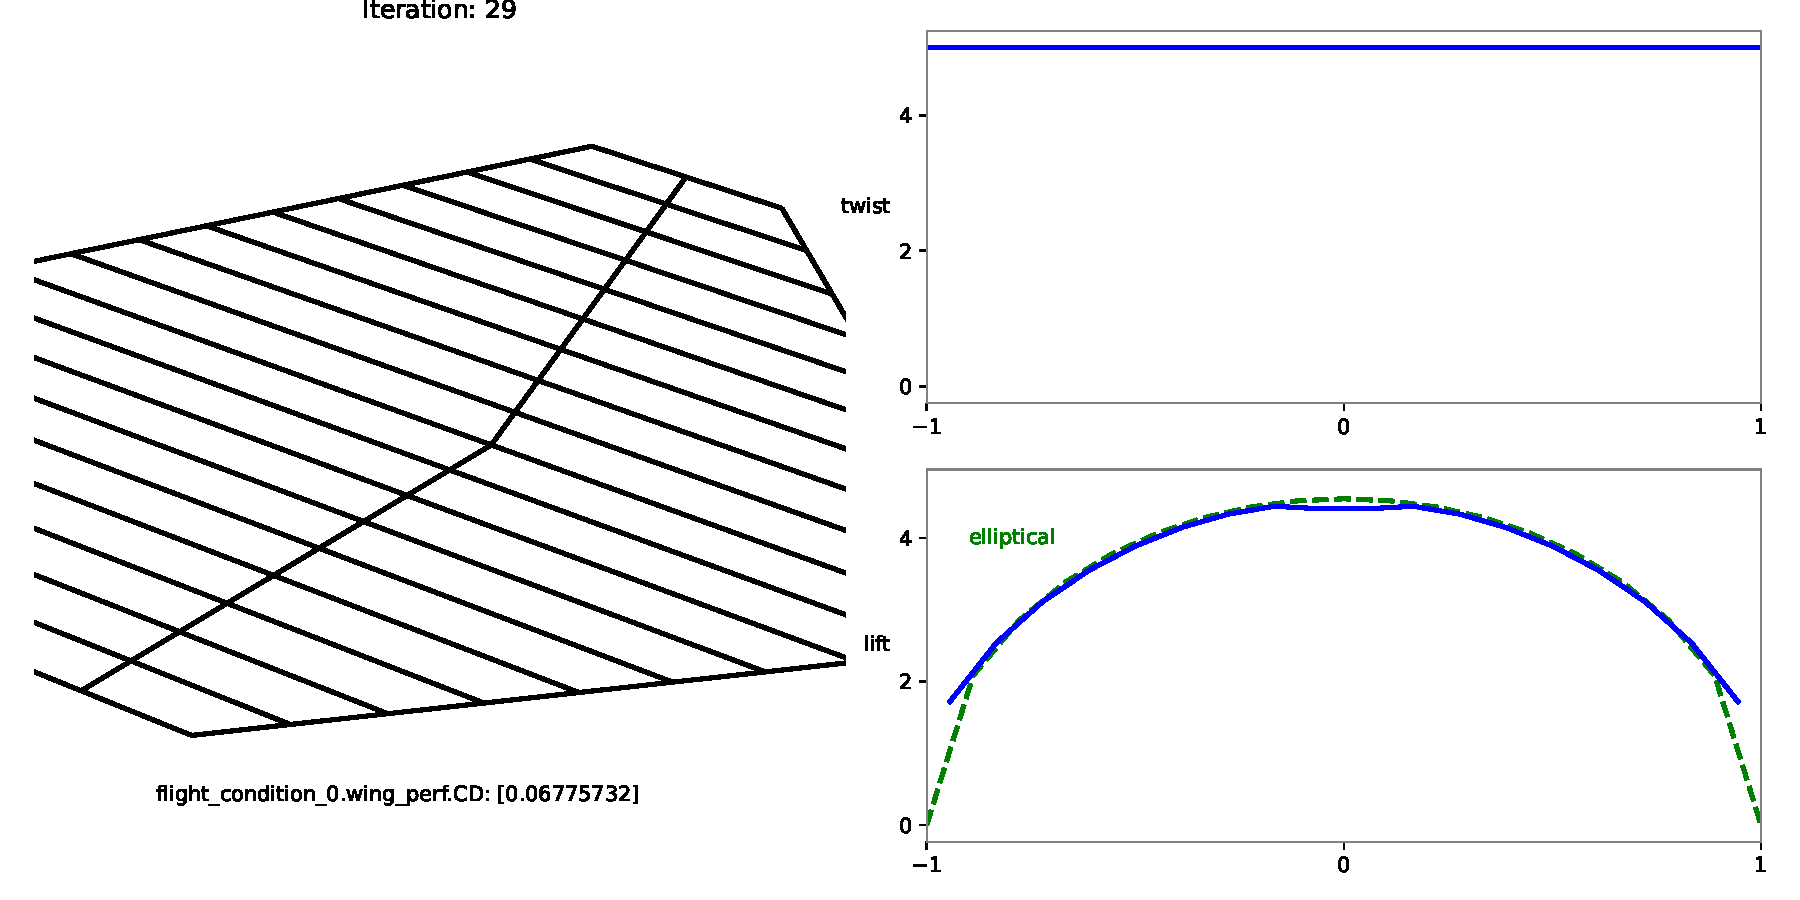
\includegraphics[width=0.75\textwidth]{/Users/conan/Desktop/LLM_Aerospace_Research/LLM_OpenAeroStruct/Figures/Optimized_Wing.pdf}
    \caption{Optimized Wing Geometry and Lift Distribution}
    \label{fig:optimized_wing}
\end{figure}

Figure \ref{fig:optimized_wing} shows the optimized wing geometry and the elliptical lift distribution. The visualization of the wing design after optimization is shown in this figure.


\end{document}